\documentclass[11pt,a4paper]{article}
\usepackage[margin=2.5cm]{geometry}
\usepackage[T1]{fontenc}
\usepackage{lmodern}
\usepackage{amsmath,amssymb}
\usepackage{graphicx}
\usepackage{booktabs}
\usepackage[numbers,sort&compress]{natbib}
\usepackage[font=small,labelfont=bf]{caption}
\usepackage{xurl}
\DeclareRobustCommand{\code}[1]{\path{#1}}
\usepackage[colorlinks=true,allcolors=blue]{hyperref}
\emergencystretch=2em
\renewcommand{\thesection}{S\arabic{section}}
\renewcommand{\thetable}{S\arabic{table}}
\renewcommand{\thefigure}{S\arabic{figure}}
\renewcommand{\theequation}{S\arabic{equation}}

\title{Electronic supplementary material for\\[4pt]
\large Modeling plant tissues with recursive spatial divisions}
\author{Alexei Vazquez}
\date{}

\begin{document}
\maketitle

\section{Image-to-network validation}
\label{sec:validation}

\paragraph{Fluorescence route.} Model networks of 300 and 800 walls (recursive division,
Gilbert tessellation, and freely crossing rods) were rendered at $1024^2$ pixels with
Gaussian blur of $1.5$ pixels and additive noise, then processed as the actin images. The
T share among three-arm junctions is $0.87$--$0.97$ for recursive-division and Gilbert
networks, and four-way crossings per junction are $0.04$--$0.06$, against $0.16$--$0.32$ for
crossing rods. The contact tail is undercounted, $P(k\geq4)=0.15$--$0.17$ against true
values $0.27$--$0.31$, and the largest degree is about one third of the true one, so exponents
estimated from fluorescence images are biased upward (\code{images/validate.py},
\code{results/pipeline_validation.txt}).

\paragraph{Label-image route.} Model tissues of 1000 cells were rasterised and processed as
the meristems. For recursive division with random cuts the recovered contact network has
$P(k\geq4,8,16)=0.30,0.085,0.023$ against true $0.29,0.085,0.026$, mean clustering $0.36$
against $0.38$, and $3.97$ geometric corners per cell against $4$; for balanced cuts the
recovered clustering is $0.03$ (\code{images/validate_tissue.py},
\code{results/validate_tissue.txt}).

\section{Parallel division}
\label{sec:parallel}

With $N=2\times10^4$ walls and three realisations per value, $\Pi=10^{-3}$ to $10^3$ gives
$\gamma=2.82$--$2.87$ (maximum likelihood, $k\geq10$), $\langle C\rangle=0.376$,
$C(k)\sim1/k$, a triangle-closure probability of $0.49$ per new wall and a correlation of
$0.94$ between $k-2$ and the product of length and age, as in sequential division. At
$\Pi=10^4$ the largest degree is $65$, against $281$ at $\Pi=10^{-3}$. At $\Pi=10^6$ the
network is Gilbert-like: $\gamma=9.05$ for $k\geq10$ and $4.61$ for $k\geq6$, largest degree
$16$, $\langle C\rangle=0.26$. The crossover rank gives $n^*/\Pi^{2/3}=0.024$, $0.038$ and
$0.055$ for $\Pi=10^3$, $10^4$ and $10^6$ (\code{model/pargrow.py},
\code{model/scan.py}, \code{model/crossover.py}, \code{results/scan_N20000.json},
\code{results/scan_N20000.txt}).

\section{Division rules}

\begin{table}[h]
\centering
\caption{Contact networks of four sequential division rules, $N=2\times10^4$ walls
(\code{model/percell.py}, \code{results/percell.txt}). $\gamma$: maximum-likelihood
exponent for $k\geq10$; $P(k\geq16)$: complementary cumulative distribution;
$\mathrm{sd}(\ln L)$: standard deviation of log wall length.}
\label{tab:rules}
\small
\begin{tabular}{@{}lccccc@{}}
\toprule
rule & $\gamma$ & $k_{\max}$ & $P(k\geq16)$ & $\langle C\rangle$ & $\mathrm{sd}(\ln L)$\\
\midrule
cell $\propto$ area, random cut & $2.90$ & $257$ & $0.022$ & $0.380$ & $0.86$\\
cell uniform, random cut & $2.89$ & $184$ & $0.021$ & $0.448$ & $3.33$\\
centroid, random angle & $2.90$ & $279$ & $0.021$ & $0.280$ & $0.69$\\
centroid, perpendicular to long axis & $3.06$ & $263$ & $0.018$ & $0.055$ & $0.59$\\
\bottomrule
\end{tabular}
\end{table}

\section{Turnover}

\begin{table}[h]
\centering
\caption{Steady states with turnover at $\Pi=0.01$, removal rate $\delta(2/\max(k,2))^s$
with $\delta$ set for about 1500 walls (\code{model/turnover.py},
\code{results/turnover_nss1500_stab*.json},
\code{results/turnover_fixed.txt}). Last row: recursive division without turnover at
$N=1500$.}
\label{tab:turnover}
\small
\begin{tabular}{@{}lccccc@{}}
\toprule
 & $n$ & $P(k\geq16)$ & $k_{\max}$ & $\langle C\rangle$ & corr$(k,\text{age})$\\
\midrule
$s=0$ (uniform) & $1481$ & $0.003$ & $22$ & $0.30$ & $0.68$\\
$s=1$ & $1438$ & $0.016$ & $60$ & $0.34$ & $0.71$\\
$s=2$ & $1456$ & $0.016$ & $75$ & $0.36$ & $0.65$\\
$s=3$ & $1583$ & $0.020$ & $67$ & $0.35$ & $0.61$\\
no turnover & $1500$ & $0.021$ & $82$ & -- & --\\
\bottomrule
\end{tabular}
\end{table}

With uniform removal the largest degree is $18$, $22$ and $27$ for steady states of $300$,
$1500$ and $4000$ walls, and $P(k\geq16)=0.003$--$0.008$ with $k_{\max}=22$--$26$ for
$\Pi=0.01$, $100$ and $3000$ at 1500 walls.

\section{Shoot meristems}

Of 1117 divisions in low-slope regions of the six plants, 672 have both hosts identified.
At the first observation after division ($0$--$4$~h) the junction angle has quartiles
$135^\circ$, $143^\circ$ and $151^\circ$, and $3.6\%$ of angles exceed $165^\circ$. The
fraction of tracked cells dividing per 4~h interval ranges from $6.4\%$ to $12.2\%$, giving
$T_{cc}=24$--$45$~h (median $36$~h). Over 12182 observations of interior low-slope cells the
fraction of cells with $n=3,\dots,9$ sides is $0.003$, $0.041$, $0.267$, $0.408$, $0.230$,
$0.046$, $0.003$; $n_1+n_2-n$ has mode $4$ in every plant, with values $5$ and $6$ when a
neighbour divides in the same interval. In $80$~h the largest observed number of contacts
of a line is $6$, and only four divisions have both hosts born during the film
(\code{images/meristem.py}, \code{images/meristem_topo.py},
\code{results/meristem_plant*.json}, \code{results/meristem_topo.json},
\code{images/corner_detector_check.py}, \code{results/corner_detector_check.txt}).

\section{Plant division model}

\begin{table}[h]
\centering
\caption{Root-mean-square deviation (degrees) between model and shoot-meristem medians of
the junction angle against age ($0$--$40$~h), for initial tension $t_0$ and maturation time
$\tau$; two realisations of 600 cells (\code{model/fit_tension.py},
\code{results/fit_tension.txt}).}
\label{tab:fit}
\small
\begin{tabular}{@{}lcccc@{}}
\toprule
 & $\tau=8$~h & $24$~h & $48$~h & $96$~h\\
\midrule
$t_0=0.30$ & $6.2$ & $8.9$ & $12.7$ & $13.7$\\
$t_0=0.45$ & $5.1$ & $5.3$ & $8.1$ & $8.2$\\
$t_0=0.60$ & $5.6$ & $1.9$ & $3.1$ & $3.4$\\
$t_0=0.75$ & $6.9$ & $3.4$ & $1.7$ & $2.6$\\
\bottomrule
\end{tabular}
\end{table}

\begin{table}[h]
\centering
\caption{Area stiffness $K$ at $t_0=0.7$, $\tau=36$~h, 1000 cells (\code{model/stiff.py},
\code{results/stiff.txt}). The linked-host fraction here is computed over all divisions,
without the observation conditions of the flower films.}
\label{tab:stiff}
\small
\begin{tabular}{@{}lcccc@{}}
\toprule
$K$ & side distribution, distance from data & angle rms & linked-host fraction\\
\midrule
$20$ & $0.095$ & $2.1^\circ$ & $0.31$\\
$100$ & $0.054$ & $3.9^\circ$ & $0.27$\\
$500$ & $0.075$ & $11.2^\circ$ & $0.41$\\
$2000$ & $0.135$ & $35.2^\circ$ & $0.45$\\
\bottomrule
\end{tabular}
\end{table}

Model networks of 2000 cells (two realisations; \code{model/predict_plant.py},
\code{results/plant_predictions_N2000.json}, \code{results/plant_predictions.txt},
\code{model/pn_distance.py}, \code{results/pn_distance.txt}) give, for Errera division
with tension maturation and cells chosen $\propto A^4$: $\gamma=2.84$ ($k\geq6$),
$\langle C\rangle=0.23$, $C(k)=0.34$, $0.16$, $0.10$, $0.07$, $0.05$, $0.03$ in degree bins
starting at $2$, $3$, $5$, $8$, $13$, $21$, and side-distribution distance $0.107$; with
cells chosen $\propto A$: $\gamma=2.94$, $\langle C\rangle=0.20$, distance $0.162$; without
relaxation: $\gamma=3.01$, $\langle C\rangle=0.0008$, distance $0.033$; random cuts:
$\gamma=2.86$, $\langle C\rangle=0.36$, corner-cut fraction $0.21$, three-sided cells
$0.09$, distance $0.370$.

\section{Flower meristems}

Six films of Refahi \textit{et al.}: FM1 ($0$--$132$~h), FM5 ($16$--$173$~h) and four
shorter films ($55$--$69$~h), with intervals of 4--13~h. 3008 new L1 walls have identified
host relations; the cell cycle from summed intervals over summed $\log_2$ daughter numbers
is $T_{cc}=31.4$~h. Of 47 divisions for which the linked-host relation is decidable, 9 have
linked hosts. Model values use $t_0=0.7$, $\tau=36$~h, $T_{cc}=31$~h over a $150$~h window:
linked-host fraction $0.190$ ($K=20$, $n=1324$), $0.187$ ($K=100$, $n=1323$) and $0.002$
without relaxation ($n=1530$). Under the model value $0.19$, observing 9 or fewer linked
hosts in 47 has probability $0.60$; under $0.002$, observing 9 or more has probability
$7\times10^{-16}$ (\code{images/refahi.py}, \code{images/refahi_stats.py},
\code{model/refahi_model.py}, \code{results/refahi_FM*.json},
\code{results/refahi_stats.json}, \code{results/refahi_model.json},
\code{results/refahi.txt}).

\begin{table}[h]
\centering
\caption{Flower meristems against the plant model ($K=20$). Junction angle: median through
angle at new junctions. Contacts: mean number of contacts of film-born lines with known
hosts; the last model bin is $110$--$150$~h.}
\label{tab:refahi}
\small
\begin{tabular}{@{}lccccccc@{}}
\toprule
age (h) & $0$--$8$ & $8$--$16$ & $16$--$24$ & $24$--$36$ & $36$--$48$ & $48$--$72$ & $72$--$120$\\
\midrule
angle, data & $135.7^\circ$ & $131.4^\circ$ & $129.9^\circ$ & $126.9^\circ$ & $125.3^\circ$ & $126.0^\circ$ & $124.3^\circ$\\
angle, model & $139.3^\circ$ & $135.0^\circ$ & $131.8^\circ$ & $128.5^\circ$ & $125.8^\circ$ & $123.2^\circ$ & $121.2^\circ$\\
\midrule
age (h) & $0$--$20$ & $20$--$40$ & $40$--$70$ & $70$--$110$ & $110$--$200$ & & \\
\midrule
contacts, data & $2.38$ & $3.07$ & $3.84$ & $3.14$ & $2.84$ & & \\
contacts, model & $2.04$ & $2.69$ & $3.50$ & $5.0$ & $8.2$ & & \\
\bottomrule
\end{tabular}
\end{table}

Beyond $70$~h the data lines are censored: walls that later abut them belong to cells outside
the tracked L1 region. The largest observed number of contacts is $12$.

\section{Leaf veins}
\label{sec:veins}

The 44 samples are those of one plot in the LeafVeinCNN release~\cite{xu2021,blonder2020}.
Of the vein nodes, $34\%$ are free ends. At interior three-way nodes of the loop network the
largest angle between arms has median $147^\circ$, and $32\%$ exceed $155^\circ$. At all
three-way nodes of the loop network the arm opposite the widest gap is the thinnest in $71\%$
of 67926 nodes; at geometric T junctions the stem is the thinnest in $78\%$
(\code{images/venation.py}, \code{images/venation_angles.py},
\code{results/venation_angles.txt}).

\paragraph{Loop nesting.} Over 20112 fusions the smaller-part fraction has mean $0.28$ and
quartiles $0.16$, $0.30$, $0.41$. Recursive division with birth-ordered widths gives a
uniform distribution on $[0,1/2]$ (mean $0.25$); centroid and balanced cuts give means
$0.47$ and $0.48$. A Voronoi tiling with random widths and recursive division with noisy
widths have lower quartiles $0.047$ and $0.076$ (\code{images/hld_null.py}).

\paragraph{Width-continuation lines.} On the leaf loop networks, continuing the two widest
arms through each node gives $P(k\geq4,8,16)=0.31$, $0.066$, $0.008$; $C(k)=0.43$, $0.24$,
$0.15$, $0.09$, $0.05$, $0.03$ in degree bins starting at $2$, $3$, $5$, $8$, $13$, $21$; and
a partial correlation of $0.40$ between $\ln k$ and $\ln W$ at fixed $\ln L$, with $W$ the
width and $L$ the length of a line (\code{images/venation_width.py}). The same
construction gives, on a Voronoi tiling with random widths, $P(k\geq4)=0.30$, $C(k)$ from
$0.34$ to $0.04$ and partial correlation $0.32$; on recursive division with random widths
$0.34$; and on recursive division with birth-ordered widths $0.57$
(\code{images/width_lines_null.py}, \code{results/width_lines_null.txt}). The
contact law and $C(k)$ are produced by the line construction; only the width--degree
correlation lies slightly above the random-width nulls.

\section{Actin in spread cells}

\begin{figure}[h]
\centering
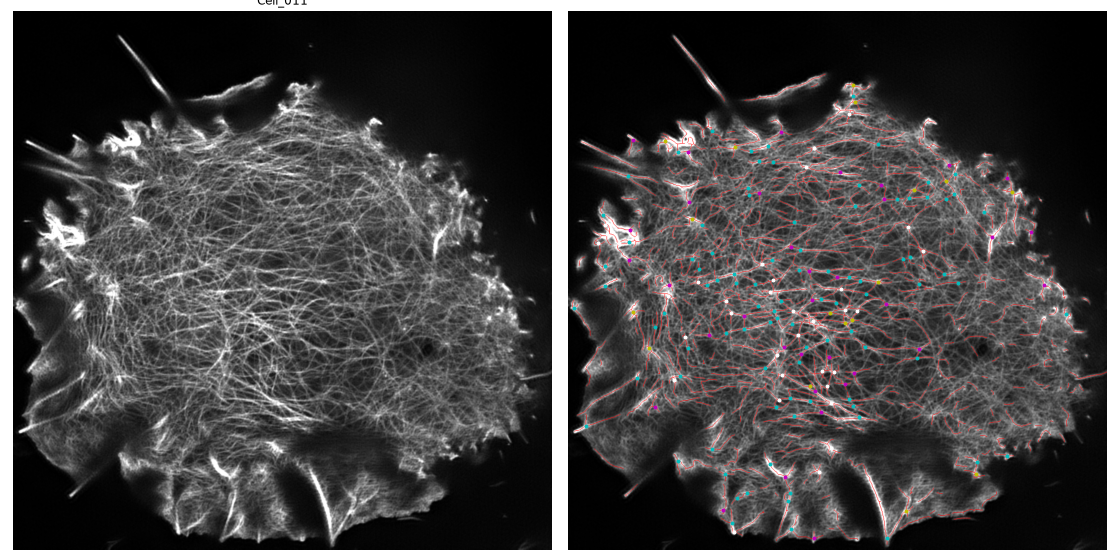
\includegraphics[width=\textwidth]{figs/figS1.png}
\caption{F-actin in a COS-7 cell (BioSR Cell\_011, Lifeact, TIRF-SIM, field $31~\mu$m).
Left: image. Right: skeleton (red) with T (cyan), Y (magenta) and four-way crossing
(yellow) junctions. Long bundles cross at shallow angles over a dense meshwork.}
\label{fig:actin}
\end{figure}

Over 51 cells the pipeline finds 11389 junctions: 4192 T, 2652 Y, 772 four-way crossings and
about 1900 clusters with five or more arms. The skeleton is fragmented (62791 line pieces,
$P(k\geq2)=0.07$), and the partial correlation between degree and bundle width at fixed
length is $0.05$ (\code{images/run_biosr.py}, \code{results/biosr_summary.json}). The
segmentation was not tuned and the cells are not human, so this result is a first pass.
Keratin networks have a mean vertex degree of $3.5$--$4.2$~\cite{luck2010}, above the value
$3$ of a partition by T junctions. Tracing algorithms that stop a curve when it meets
another, such as SOAX~\cite{xu2015soax}, create T junctions by construction. Cortical actin
compartments, whose areas are log-normal and have been interpreted as successive
fragmentation by growing filaments~\cite{sadegh2017}, are the closest published analogue.

\section{Code and results}

All code and results are in the folder \code{bio/} of
\url{https://github.com/av2atgh/scalerich}. Python scripts run with the environment described
in \code{bio/NOTES.md}; figures are produced by \code{figures.py}. Each section above
names the scripts and the result files from which its numbers are read.

\bibliographystyle{unsrtnat}
\bibliography{references}

\end{document}
